
\section{Results}

Participants reached towards the target object after it appeared, `spawned', on the table. In the match trials without visuo-tactile glitches, participants took on average 1.04s (SD = .19) to complete the reach-to-touch. In the mismatch trials with visuo-tactile glitches, the target feedback was presented prematurely and triggered on average after .73s (SD = .12) following object spawn, see figure 1b. Hence, increasing the (bounding) object volume for collision detection led to a spatio-temporal mismatch of approximately 300 ms as compared to the congruent condition. The velocity profile in both conditions exhibited a narrow peak during outward reaching with a peak magnitude of ~.6 m/s and a broader and lower peak when the hand was retracted back to its origin, see figure \ref{setup_and_behavior}b bottom.

\begin{figure}[!h]
  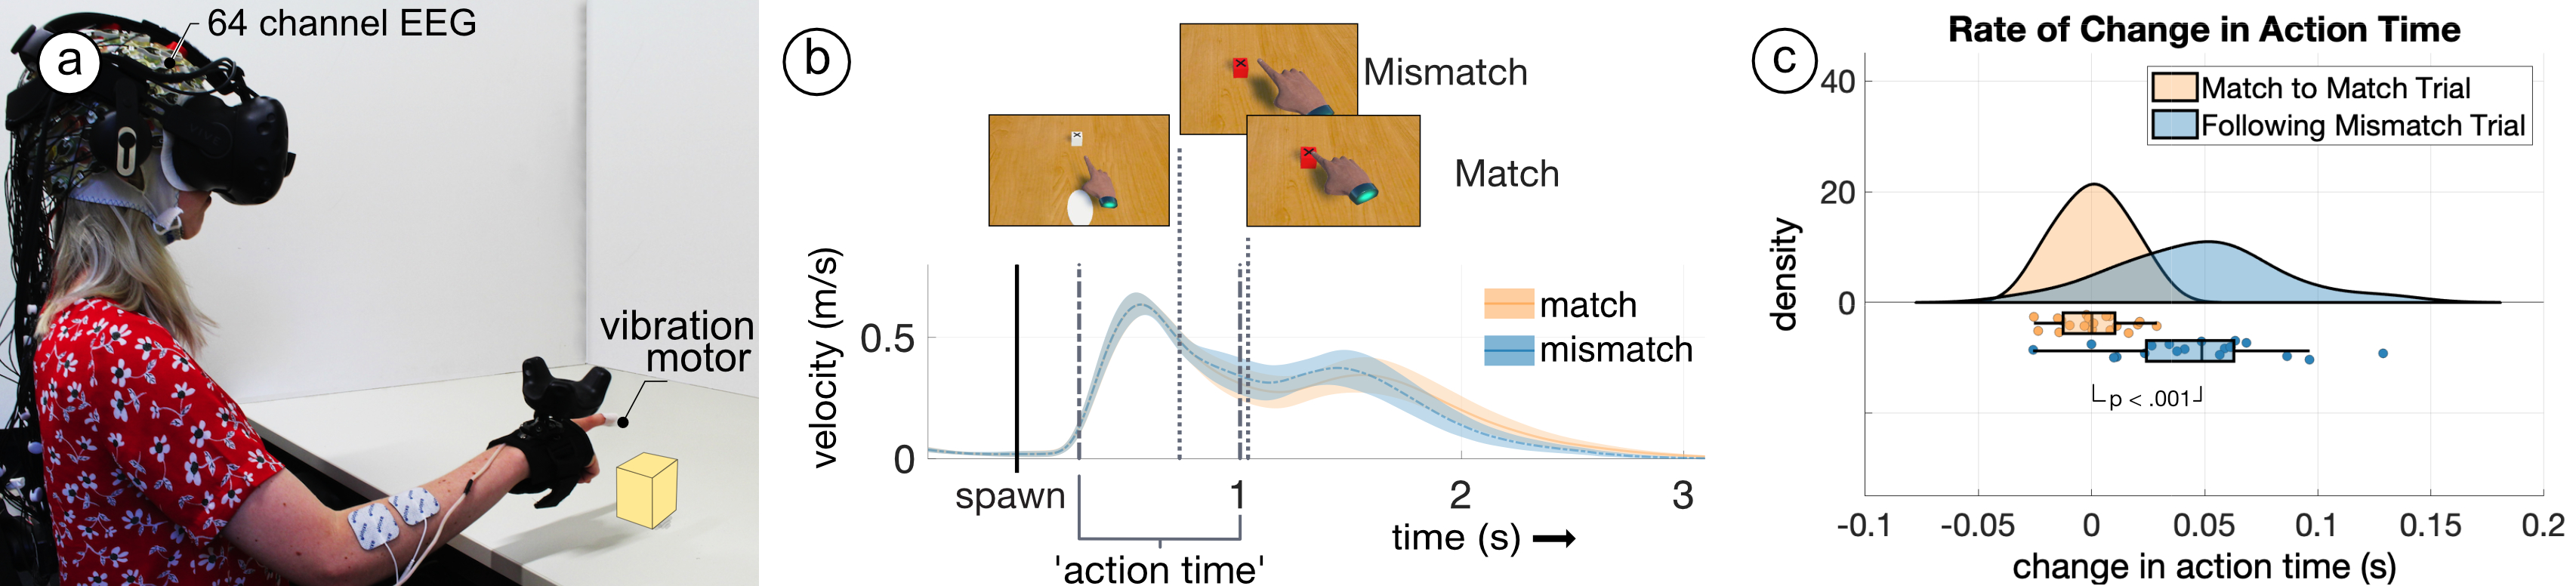
\includegraphics[width=\textwidth]{figures/task_behavior.jpg}
  \caption{Task Structure and hand velocity profile. \textbf{A} Participants were instructed to reach to an appearing cube on a desk in front of them. They were equipped with a VR, a 64 channel EEG cap, electrode spacers and rigid body tracker on the hand. The vibration motor was placed under the fingertip of the index finger. \textbf{B} Top: Inside VR view of experimental scene. Bottom: Grand-average velocity with 95\% confidence interval of both, match and mismatch conditions with event markers for object `spawn', `action time' start and end as well as moments of object touch in match and mismatch conditions. \textbf{C} Distribution of \textit{rate of change} in `action time' between two subsequent match trials and following a VR glitch. A dot represents the average per participant per condition.}
  \label{setup_and_behavior}
\end{figure}

\subsection{Prolonged `Action time' Following VR Glitches}

`Action time', the hand movement period from movement start to reaching the object, lasted on average .74s (SD = .15) in match- and .69s (SD = .15) in mismatch trials. 

% Adding vibrotactile stimulation did not affect hand movement profiles ($b=-.01, t=-1.7, p=.1$) and neither did the interaction of congruity and vibrotactile stimulation ($b=.02, t=1.8, p=.07$). Hence, as with the EEG analysis we pooled trials ignoring the feedback modulation.

We calculated the \textit{rate of change} in `action time' as a metric of post-error slowing. Following match trials, `action time' in the subsequent trial did not change, i.e. 0s (SD = .02). However, following mismatch trials, `action time' was increased in the subsequent trial on average by .05s (SD = .04); this modulation was about 48 times more likely to occur under the model considering mismatch modulation than the null model (equivalent ${\chi}^2_{(1)} = 48.1, p<.001$), see figure \ref{setup_and_behavior}c. 

% Adding vibrotactile feedback did not affect post-error slowing significantly ($b=-.02, t=-1.4, p=.15$). 

Using the trial-to-trial adaptation in `action time', trial classes (match/mismatch) were classified with an average within-subject classification accuracy across folds of 55.4\% (SD = 4.8), remaining below the significance threshold of the simulated chance level at 63.4\% (SD = 0.6).

\footnote{For completeness, we also report a classification scheme using behavioral data of all trials, maintaining unequal trial numbers per match and mismatch condition. We found that using data from all trials and maintaining unequal class sizes increased the classification to 67\% accuracy. See the supplementary material for more detail.}









%%%% writing resources
% Frage: wenn vel profiles mit movement onset aligned dann sollten evtl. kurven gleich sein, es sei denn es gibt einen "kontinuierlichen" rekalibrationseffekt ist in den syncs. mit drin
% im idealfall ist der rekalibrationseffekt 1/4 der 300ms
% Optimierungsprozess um den RMSE bei rekalibration zu optimieren
% mallot VR noise adaptation
% The addition of a haptic sensation while touching the virtual objects (by means of vibrotactile stimulation) led participants to generally move their hand slower during the whole trial, see \ref{setup_and_behavior} C middle row. Participants started their outward movement earlier and their outward peak magnitude was lower when approaching the target (for example at 50 ms preceding object selection, $t_{18} = -2.14, P = .03$). Following trials with spatio-temporal asynchrony, movement behavior was altered in the next trial. An earlier movement onset with a broader peak and immediate retraction following object select was observed (for example at 100 following object selection, $t_{18} = -17.24, P = 0$). Taken together, the task introduced spatio-temporal asynchrony, with rendered vibrotactile feedback as well as the asynchrony impacting future reaching movement characteristics.